\documentclass[11pt,a4paper,twoside,french,svgnames]{report}
\usepackage[utf8]{inputenc} % force the use of utf8
\usepackage[T1]{fontenc} % font encoding, allows accents (T1 font encoding is an 8-bit encoding)
\usepackage[top=2.5cm,bottom=2.5cm,outer=2.5cm,inner=2.5cm]{geometry} % http://tex.stackexchange.com/questions/62311/a4paper-where-should-i-declare-it-in-document-class-or-geometry // another option: papersize={21cm,29.7cm}
\usepackage[french]{babel} % translate everything in the desired language: table of contents, etc. 'english' can be replaced with 'francais'
\usepackage{graphicx} % images management
\usepackage{wrapfig} % floating images
\usepackage[format=plain,labelfont=bf,font=small,justification=centering,margin=10pt]{caption} % allow multiline captions in figures,
\usepackage{float} % allow \begin{figure}[H] and \begin{table}[H] (to really force positionning, unlike h!)
\usepackage{array} % allow arrays
\usepackage[super]{nth} % allow to write \nth(1) to write 1st, etc
\usepackage{fancyhdr} % headers/footers management (overrides empty, plain and headings)
\usepackage{upquote} % without this, lslisting replace vertical singles quotes with curved ones
\usepackage{listings} % code insertion (MUST BE WRITTEN AFTER BABEL)
\usepackage[
            backend=biber,
            style=numeric,
            sorting=none, % nty = name title year
            url=true, % always show url when provided
            ]{biblatex}
%\usepackage{pdfpages} % include PDF documents
\usepackage{enumitem} % for /setlist
\usepackage{color,soul} % add some colors and hightlight
\usepackage{xcolor} % more colors
\usepackage{afterpage} % allow to execute command after the current page ends
\usepackage[hidelinks,
            colorlinks  = true, % no borders, colors enabled
            anchorcolor = blue,
            linkcolor   = black, % links in table of contents
            urlcolor    = blue,
            citecolor   = blue,
            breaklinks  = true]{hyperref}
\newcommand{\MYhref}[3][blue]{\href{#2}{\color{#1}{#3}}}%

% List settings
\setlist{itemsep=.5em}
\setlist[itemize,2]{label={$\bullet$}} % use bullets for nested itemize in level 2

% REQUIRE
% \usepackage{color}
% \usepackage{listings} % (MUST BE WRITTEN AFTER BABEL)

% General colors
\definecolor{comment}{rgb}{0.12, 0.38, 0.18 } % adjusted, in Eclipse: {0.25, 0.42, 0.30 } = #3F6A4D
\definecolor{keyword}{rgb}{0.2, 0.2, 0.8}
\definecolor{string}{rgb}{0.06, 0.10, 0.98} % #101AF9

% Language-specific colors
% JavaScript
\definecolor{darkgray}{rgb}{.4,.4,.4}
%\definecolor{purple}{rgb}{0.65, 0.12, 0.82}

% hack to force UTF-8 compatibility (for french only)
\lstset{
       extendedchars=true,
       literate={à}{{\`a}}1 {â}{{\^a}}1 %                         lettre a
                {À}{{\`A}}1 {Â}{{\^A}}1 %                         lettre A
                {ç}{{\c{c}}}1 %                                   lettre c
                {Ç}{{\c{C}}}1 %                                   lettre C
                {é}{{\'e}}1 {è}{{\`e}}1 {ê}{{\^e}}1 {ë}{{\"e}}1 % lettre e
                {É}{{\'E}}1 {È}{{\`E}}1 {Ê}{{\^E}}1 {Ë}{{\"E}}1 % lettre E
                {î}{{\^i}}1 {ï}{{\"i}}1 %                         lettre i
                {Î}{{\^I}}1 {Ï}{{\"I}}1 %                         lettre I
                {ô}{{\^o}}1 %                                     lettre o
                {Ô}{{\^O}}1 %                                     lettre O
                {œ}{{\oe}}1 %                                     lettre oe
                {Œ}{{\OE}}1 %                                     lettre OE
                {ù}{{\`u}}1 {û}{{\^u}}1 {ü}{{\"u}}1 %             lettre u
                {Ù}{{\`U}}1 {Û}{{\^U}}1 {Ü}{{\"U}}1 %             lettre U
}

% General rules
\lstset{
  rulecolor=\color{black!50},
  backgroundcolor = \color{blue!10},
  numbers=none, %left % display line numbers
  showspaces=false,
  showtabs=false,
  breaklines=true,
  showstringspaces=false,
  breakatwhitespace=false,
  commentstyle=\color{comment},
  keywordstyle=\color{keyword},
  stringstyle=\color{string},
  basicstyle=\ttfamily,
  extendedchars=true,
  emph=[2]{In},
  emphstyle=[2]\color{black!70},
  morecomment=[l][\color{blue}]{Out},
  frame=single,
  frameround=tttt,
  framerule=0.3pt,
  framesep=4pt,
  belowcaptionskip=2.1pt
}

% % Define "Javascript" because lstlistings doesn't know it
% Taken from https://gist.github.com/Geruhn/3d21f60a869457373d84
\lstdefinelanguage{javascript}{
  keywords={break, case, catch, continue, debugger, default, delete, do, else, false, finally, for, function, if, in, instanceof, new, null, return, switch, this, throw, true, try, typeof, var, void, while, with},
  morecomment=[l]{//},
  morecomment=[s]{/*}{*/},
  morestring=[b]',
  morestring=[b]",
  ndkeywords={class, export, boolean, throw, implements, import, this},
  %keywordstyle=\color{blue}\bfseries,
  ndkeywordstyle=\color{darkgray}\bfseries,
  identifierstyle=\color{black},
  %commentstyle=\color{purple}\ttfamily,
  %stringstyle=\color{red}\ttfamily,
  sensitive=true
}

% Usage: \javascript
\newcommand{\javascript}{\lstset{
  language=javascript,
  title={{\setlength{\fboxsep}{1pt}\fcolorbox{orange}{yellow!20}{\sffamily\scriptsize
              \textcolor{gray!10}{\_}JavaScript\textcolor{gray!10}{\_}}}}
  }
}

% Usage: \code{My title}
\newcommand{\code}[1]{\lstset{
  language=,
  title={{\setlength{\fboxsep}{1pt}\fcolorbox{orange}{yellow!20}{\sffamily\scriptsize
              \textcolor{gray!10}{\_}{#1}\textcolor{gray!10}{\_}}}}
  }
}

% Usage: \sql
\newcommand{\sql}{\lstset{
  language=SQL,
  title={{\setlength{\fboxsep}{1pt}\fcolorbox{orange}{yellow!20}{\sffamily\scriptsize
              \textcolor{gray!10}{\_}SQL\textcolor{gray!10}{\_}}}}
  }
}

% Usage: \fakeshell
\newcommand{\fakeshell}{\lstset{
  language=bash
  }
}

\newcommand{\java}{\lstset{
  language=java,
  title={{\setlength{\fboxsep}{1pt}\fcolorbox{orange}{yellow!20}{\sffamily\scriptsize
              \textcolor{gray!10}{\_}Java\textcolor{gray!10}{\_}}}}
  }
}

\newcommand{\perl}{\lstset{
  language=perl
  }
}

\newcommand{\xml}{\lstset{
  language=xml
  }
}

% REQUIRES
% Nothing

% Redefine chapter titles: only display the title and remove useless blank space
% Original "/usr/share/texlive/texmf-dist/tex/latex/base/report.cls" edited
\makeatletter
  \def\@makechapterhead#1{% chapter{}
  \vspace*{0\p@}% 50 before
  {\parindent \z@ \raggedright \normalfont
    %\ifnum \c@secnumdepth >\m@ne
    %    \huge\bfseries \@chapapp\space \thechapter
    %    \par\nobreak
    %    \vskip 20\p@
    %\fi
    \interlinepenalty\@M
    \Huge \bfseries \thechapter\quad #1   
    \vskip 40\p@
  }}
  \def\@makeschapterhead#1{% chapter*{}
  \vspace*{0\p@}% 50 before
  {\parindent \z@ \raggedright
    \normalfont
    \interlinepenalty\@M
    \Huge \bfseries  #1\par\nobreak
    \vskip 40\p@
  }}
\makeatother
% REQUIRES
% \usepackage{fancyhdr} % headers/footers management (overrides empty, plain and headings)

% THE ORDER IS REALLY IMPORTANT, OTHERWISE IT WILL BREAK THINGS

% 1.
% Redefines the existing 'plain' style, (because 'chapter' and \tableofcontents ignores the page style currently in effect for their first page)
\fancypagestyle{plain}{
    % Took from: http://anorien.csc.warwick.ac.uk/mirrors/CTAN/macros/latex/contrib/fancyhdr/fancyhdr.pdf
    \fancyhead[LO,RE]{\slshape \leftmark}
    \fancyhead[LE,RO]{\slshape \rightmark}

    % Footers
    \renewcommand{\footrulewidth}{0.4pt}
    \fancyfoot[C]{Rapport de TD -- Steve \textsc{Lagache} \& Romain \textsc{Pellerin}}
    \fancyfoot[LE,RO]{\ifdefined\thepage \thepage \fi} % to be used with \pagenumbering{gobble} % no numerotation
    % \fancyfoot[LE,RO]{\ifnum\thepage>0 \thepage \fi} % to be used with %\addtocounter{page}{-4} % numerotation begins at 1 + (-4)
}

% 2.
\pagestyle{plain}

% 3.
% http://tex.stackexchange.com/questions/111223/markboth-is-not-working-when-using-chapter-and-section
% Took from : http://ftp.snt.utwente.nl/pub/software/tex/macros/latex/contrib/fancyhdr/fancyhdr.pdf
\renewcommand{\chaptermark}[1]{\markboth{}{\MakeUppercase{\thechapter.\ #1}}}
\renewcommand{\sectionmark}[1]{}

% NORMALLY
% \renewcommand{\chaptermark}[1]{\markboth{\MakeUppercase{\thechapter.\ #1}}{}}
% \renewcommand{\sectionmark}[1]{\markright{\thesection.\ #1}}
 % To be edited to change the header and footer

\title{Rapport de TD}
\author{Steve LAGACHE et Romain PELLERIN}
\date\today
\setcounter{tocdepth}{2} % ToC depth

\pagenumbering{arabic} % re-enable numering

\begin{document}
\thispagestyle{empty} % only applies to this page
\begin{center}

\includegraphics[height=3cm]{images/logo-utc.png}

\vspace{4cm}

\noindent{\LARGE\MYhref[black]{http://www.utc.fr/}{Université de Technologie de Compiègne}}

\vspace{1cm}

{\large Génie Informatique}

\vspace{3cm}
\noindent\fbox{
\begin{minipage}{.9\textwidth}
\begin{center}
    \vspace{0.3cm}\Large{Rapport de TD}\\
    \vspace{0.3cm}\LARGE{\textbf{LO17}}\vspace{0.3cm}\\
\end{center}
\end{minipage}}

\vspace{3cm}

\begin{tabular}{>{\hfill\arraybackslash}p{5cm}p{5cm}}
%\hline
    \multicolumn{2}{c}{\textbf{Steve \textsc{LAGACHE} \& Romain \textsc{PELLERIN}}}\\\\
%\hline
    \multicolumn{2}{c}{Chargé de TD : Pierre \textsc{Morizet-Mahoudeaux}}\\\\
%\hline
    \multicolumn{2}{c}{Printemps 2016 (P16)}\\
%\hline

\end{tabular}
\vfill

{\footnotesize Dernière mise à jour: \today}
\end{center}


\tableofcontents

\chapter{XML}

\section{Arbre}

Voici un exemple d'arbre XML illustrant les données manipulées pour ce projet.

\xml
\begin{lstlisting}
<?xml version = "1.0" encoding="UTF-8" standalone="yes" ?>
<annuaire>
	<annuaire_id>Id</annuaire_id>
	<categorie categorie_id ="Id" name="categorie">
		<annonce>
			<annonce_id>Id</annonce_id>
			<nom>Nom</nom>
			<adresse>
				<adresse_id>Id</adresse_id>
				<rue>Rue</rue>
				<ville>Ville</ville>
				<codepostal>00000</codepostal>
			</adresse>
			<telephone>0000000000</telephone>
		</annonce>
		<annonce>
			<annonce_id>Id</annonce_id>
			<nom>Nom</nom>
			<adresse>
				<adresse_id>Id</adresse_id>
				<rue>Rue</rue>
				<ville>Ville</ville>
				<codepostal>00000</codepostal>
			</adresse>
			<telephone>0000000000</telephone>
		</annonce>
	</categorie>
	<categorie categorie_id ="Id" name="categorie">
		<annonce>
			<annonce_id>Id</annonce_id>
			<nom>Nom</nom>
			<adresse>
				<adresse_id>Id</adresse_id>
				<rue>Rue</rue>
				<ville>Ville</ville>
				<codepostal>00000</codepostal>
			</adresse>
			<telephone>0000000000</telephone>
		</annonce>
	</categorie>
</annuaire>
\end{lstlisting}
Et voici sa représentation graphique sous forme d'arbre :
\begin{figure}[H]
    \centering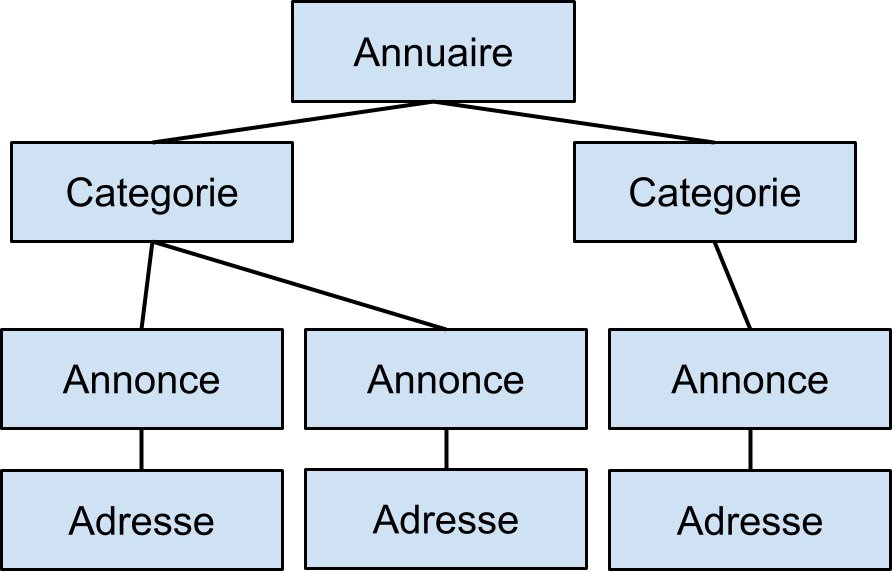
\includegraphics[width=.7\textwidth]{images/arbre.png}
    \caption{Arbre de l'XML}
\end{figure}

\section{Schéma XML}

Voici le schéma XSD correspond à notre XML :

\begin{lstlisting}
<?xml version="1.0" encoding="UTF-8" ?>
<xs:schema attributeFormDefault="unqualified" elementFormDefault="qualified" xmlns:xs="http://www.w3.org/2001/XMLSchema">
  <xs:element name="annuaire">
    <xs:complexType>
      <xs:sequence>
        <xs:element type="xs:string" name="annuaire_id"/>
        <xs:element name="categorie" maxOccurs="unbounded" minOccurs="0">
          <xs:complexType>
            <xs:sequence>
              <xs:element name="annonce" maxOccurs="unbounded" minOccurs="0">
                <xs:complexType>
                  <xs:sequence>
                    <xs:element type="xs:string" name="annonce_id"/>
                    <xs:element type="xs:string" name="nom"/>
                    <xs:element name="adresse">
                      <xs:complexType>
                        <xs:sequence>
                          <xs:element type="xs:string" name="adresse_id"/>
                          <xs:element type="xs:string" name="rue"/>
                          <xs:element type="xs:string" name="ville"/>
                          <xs:element type="xs:byte" name="codepostal"/>
                        </xs:sequence>
                      </xs:complexType>
                    </xs:element>
                    <xs:element type="xs:byte" name="telephone"/>
                  </xs:sequence>
                </xs:complexType>
              </xs:element>
            </xs:sequence>
            <xs:attribute type="xs:string" name="categorie_id" use="optional"/>
            <xs:attribute type="xs:string" name="name" use="optional"/>
          </xs:complexType>
        </xs:element>
      </xs:sequence>
    </xs:complexType>
  </xs:element>
</xs:schema>
\end{lstlisting}

\chapter{Conception}
\section{Diagramme de classes}

\begin{figure}[H]
    \centering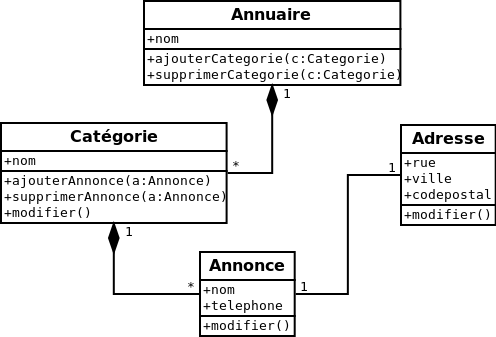
\includegraphics[width=.8\textwidth]{images/UML.png}
    \caption{Diagramme de classes (UML)}
\end{figure}

\section{Diagramme logique de données (MLD)}

\fakeshell
\begin{lstlisting}
Annuaire(#nom:string)
Categorie(#nom:string, #annuaire=>Annuaire(nom))
Annonce(#nom:string, #categorie=>Categorie(nom), adresse=>Adresse(adresse_id), telephone:string)
Adresse(#adresse_id:integer, rue:string, ville:string, codepostal:string)
\end{lstlisting}

\chapter{Web service}

\section{Interface : prototypes des méthodes}

Nous avons décidé de créer deux webservices :

\begin{itemize}
    \item Un pour l'application cliente d'administration (création, modification et suppression des catégories et annonces)
    \item Un pour l'application cliente de recherche d'annonces
\end{itemize}

Voici le webservice d'administration :

\java
\begin{lstlisting}
String createCategory(String name)

String deleteCategorie(int categorie_id)

String updateCategorie(int categorie_id, String name)

String getAllCategorie()

String getCategory(int category_id)

String createAd(String name, int categorie_id, String rue, String ville, String codepostal, String telephone)

String deleteAd(int annonce_id)

String updateAd(int annonce_id, String name, int categorie_id, String rue, String ville, String codepostal, String telephone)

String getAllAd()

String getAd(int annonce_id)
\end{lstlisting}
Et voici le webservice pour la recherche d'annonces :
\begin{lstlisting}
String getByParams(String name, String categoryName, String street, String city, String postcode)
\end{lstlisting}
Pour nos deux webservices, chaque fonction retourne une \lstinline{String} au format JSON.

\section{Messages SOAP}

\subsection{Requête}

Voici une requête faite depuis l'application cliente de recherche d'annonces, vers le serveur :

\xml
\begin{lstlisting}
<?xml version="1.0" encoding="UTF-8"?>
<soapenv:Envelope xmlns:soapenv="http://schemas.xmlsoap.org/soap/envelope/" xmlns:xsd="http://www.w3.org/2001/XMLSchema" xmlns:xsi="http://www.w3.org/2001/XMLSchema-instance">
	<soapenv:Body>
		<getByParams xmlns="http://webservice">
			<name>ad</name>
			<categoryName xsi:nil="true"/>
			<street xsi:nil="true"/>
			<city>paris</city>
			<postcode xsi:nil="true"/>
		</getByParams>
	</soapenv:Body>
</soapenv:Envelope>
\end{lstlisting}

\subsection{Réponse}

Et voici la réponse à cette requête. Nous retournons du JSON qui est encapsulé dans du XML automatiquement.

\begin{lstlisting}
<?xml version="1.0" encoding="utf-8"?>
<soapenv:Envelope xmlns:soapenv="http://schemas.xmlsoap.org/soap/envelope/" xmlns:xsd="http://www.w3.org/2001/XMLSchema" xmlns:xsi="http://www.w3.org/2001/XMLSchema-instance">
	<soapenv:Body>
		<getByParamsResponse xmlns="http://webservice">
			<getByParamsReturn>
                [{&quot;annonce_id&quot;:1,&quot;nom&quot;:&quot;ad11&quot;,&quot;categorie_id&quot;:8,&quot;adresse_id&quot;:1,&quot;telephone&quot;:&quot;0251&quot;,&quot;categorieObjet&quot;:{&quot;categorie_id&quot;:8,&quot;nom&quot;:&quot;cat2358&quot;},&quot;adresseObjet&quot;:{&quot;adresse_id&quot;:1,&quot;rue&quot;:&quot;rue&quot;,&quot;ville&quot;:&quot;paris&quot;,&quot;codepostal&quot;:&quot;85&quot;}},{&quot;annonce_id&quot;:2,&quot;nom&quot;:&quot;ad2&quot;,&quot;categorie_id&quot;:1,&quot;adresse_id&quot;:2,&quot;telephone&quot;:&quot;0251&quot;,&quot;categorieObjet&quot;:{&quot;categorie_id&quot;:1,&quot;nom&quot;:&quot;cat1&quot;},&quot;adresseObjet&quot;:{&quot;adresse_id&quot;:2,&quot;rue&quot;:&quot;rue&quot;,&quot;ville&quot;:&quot;parisss&quot;,&quot;codepostal&quot;:&quot;85&quot;}}]
			</getByParamsReturn>
		</getByParamsResponse>
	</soapenv:Body>
</soapenv:Envelope>
\end{lstlisting}

\chapter{Architecture}

\begin{figure}[H]
    \centering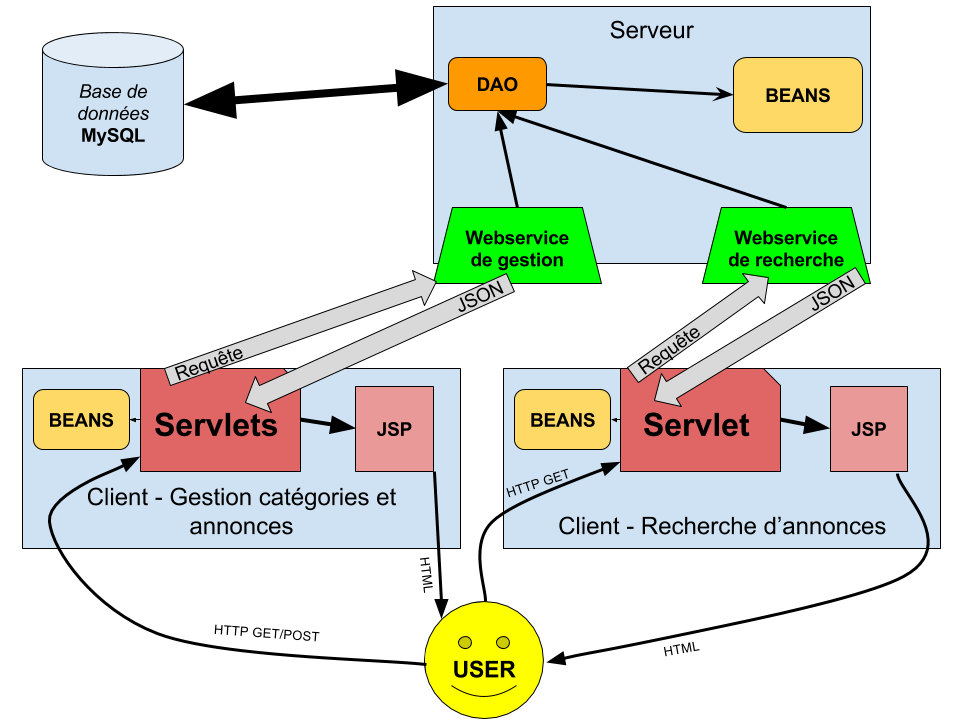
\includegraphics[width=1\textwidth]{images/archi.png}
    \caption{Architecture de l'application}
\end{figure}

Un utilisateur peut utiliser deux applications web (qui tournent sur Tomcat) au choix:
\begin{itemize}
  \item Une application web de gestion de l'annuaire, où il peut créer, modifier et supprimer des catégories. Il peut également faire la même chose avec des annonces.
  \item Une application web de consultation où il peut voir l'ensemble des annonces ou alors faire des recherches sur les annonces pour en trouver seulement certaines, répondant à des critères de recherche.
\end{itemize}

Lorsqu'il accède à l'une des deux applications, voici ce qu'il se passe :

\begin{enumerate}
  \item Il envoit une requête HTTP à l'application web pour accèder à une page.
  \item Selon les paramètres contenus dans la requête (qui peut être de type GET ou POST), la servlet va soit simplement renvoyer une page HTML générée à partir d'une page JSP, soit faire des traitements plus poussés en utilisant l'API (webservice) de notre serveur, puis renvoyer du HTML généré à partir d'une JSP et de la réponse de l'API.
  \item Dans le cas où la servlet a besoin d'utilisateur le web service, elle va utiliser un objet de la classe \lstinline{Proxy} (en appelant une méthode sur cet objet). De manière transparente, une requête est faite sur le serveur, qui tourne aussi sur Tomcat.
  \item La fonction du webservice qui est appelée va instancier une ou plusieurs DAO.
  \item Les DAO utilisent les \lstinline{Beans}, qui sont une représentation des tables SQL que nous avons créées. Les DAO vont donc faire des requêtes SQL et instancier des objets \lstinline{Beans} à partir des résultats de la requête SQL.
  \item La fonction du webservice initialement appelée récupère les résultats produits par la ou les DAO et les sérialise en JSON.
  \item Le JSON est retourné à la servlet.
  \item La servlet désérialise le JSON et instancie des \lstinline{Beans}. Ces derniers, souvent sous forme de listes, sont transmis à la JSP qui va produire le HTML renvoyé au client.
\end{enumerate}


%\chapter{Conclusion}

À travers l'intégralité de ces différents TD, nous avons pu découvrir les méthodes liées à l'indexation et la recherche de l'information étape par étape. D'abord par la structuration d'information brut en un corpus XML puis la création de tables inverses de lemmes et d'une stop list ; ensuite par un travail de réflexion et d'analyse sur la correction orthographique d'une phrase entrée par un utilisateur ; et enfin par l'analyse lexicale et syntaxique d'une requête en langage naturel à l'aide d'une grammaire SQL.

\medskip

Ces différentes étapes furent ensuite amenées à être rassemblées en une seule application, qui sert d'interface entre l'utilisateur demandant une requête et la base de données questionnée.

\medskip

L'objectif idéal pour ce projet final serait d'obtenir une application à même de traiter presque n'importe quelle requête, quelle que soit la formulation de cette dernière ou le nombre de critères demandés, en prenant en considération les fautes de frappe (et pas seulement les inversions de lettres), etc.

\end{document}
